\section{Two 4-transpositions}

\paragraph{}
If there are two 4-transpositions, there are 12 edges but the minimum number to link 11 points is 10. So there are two "joker" edges. There are three different possibilities for those "joker" edges: two double edges, one double edge and one alternating square or two alternating squares. We study this three cases.

\begin{lemma}
  If there are two double edges then they must be $(\rho_0, \rho_2)$ and $(\rho_1, \rho_3)$.
\end{lemma}

\begin{proof}
  If the difference between the indices of one double edge is not 2, this double edge must be included in an alternating square by Proposition~\ref{continue-double-edge}. But there are no alternating squares, thus the difference of the indices must be 2. There are only two possibilities: $(\rho_0, \rho_2)$ and $(\rho_1, \rho_3)$

  \paragraph{}
  If there are two double edges $(\rho_0, \rho_2)$, then all $\rho_0$ edges have been used and the graph is the following:

  \begin{figure}[H]
    \begin{center}
      \begin{tikzpicture}[scale=.8]

        \begin{scope}[every node/.style={circle,draw, transform shape}]
          \node (1)  at (0,0) {};
          \node (2)  at (2,0) {};
          \node (3)  at (4,0) {};
          \node (4)  at (6,0)  {};
          \node (5)  at (8,0)  {};
          \node (6)  at (10,0)  {};
          \node (7)  at (12,0)  {};
          \node (8)  at (18,0)  {};
          \node (9)  at (20,0)  {};
          \node (10) at (16,0)  {};
          \node (11) at (14,0)  {};
        \end{scope}

        \begin{scope}[every node/.style={fill=white, transform shape}]

          \begin{scope}[every edge/.style={draw}]
            \path (1)  edge[bend left=30] node {$0$} (2);
            \path (8)  edge[bend left=30] node {$0$} (9);
            \path (1)  edge[bend right=30] node {$2$} (2);
            \path (8)  edge[bend right=30] node {$2$} (9);
          \end{scope}
        \end{scope}

      \end{tikzpicture}
      \caption{}
    \end{center}
  \end{figure}

  \paragraph{}
  To connect the two $\rho_3$ edges, since no alternating square or double edge can be built, the $\rho_3$ edges must be surrounded by two $\rho_2$ edges by Lemma~\ref{rho0atEnd}. Hence one $\rho_3$ edge must use one of the two ends of the graph.

  \paragraph{}
  Thus at least one double edge is not placed at one end of the graph and thus needs two $\rho_2$ edges to be connected. But the last double edge also needs at least one $\rho_2$ edge. And thus 5 $\rho_2$ edges are needed but that is impossible\footnote{False}.

\end{proof}

\begin{lemma}
  If there are one double edges and one alternating square then they must be $(\rho_0, \rho_2)$ and $[\rho_1, \rho_3]$.
\end{lemma}

\begin{proof}
  If the indices of the double edge are consecutive, then this double edge must be included in an alternating square by Proposition~\ref{continue-double-edge}. If the double edge is $(\rho_0, \rho_1)$, the alternating square must be $[\rho_0, \rho_2]$.

  \begin{figure}[H]
    \begin{center}
      \begin{tikzpicture}[scale=.8]

        \begin{scope}[every node/.style={circle,draw, transform shape}]
          \node (1)  at (0,0) {};
          \node (2)  at (0,2) {};
          \node (3)  at (2,0) {};
          \node (4)  at (2,2)  {};
          \node (5)  at (4,0)  {};
          \node (6)  at (6,0)  {};
          \node (7)  at (8,0)  {};
          \node (8)  at (10,0)  {};
          \node (9)  at (12,0)  {};
          \node (10) at (14,0)  {};
          \node (11) at (16,0)  {};
        \end{scope}

        \begin{scope}[every node/.style={fill=white, transform shape}]

          \begin{scope}[every edge/.style={draw}]
            \path (1)  edge[bend left=30] node {$0$} (2);
            \path (3)  edge node {$0$} (4);
            \path (1)  edge[bend right=30] node {$1$} (2);
            \path (1)  edge node {$2$} (3);
            \path (2)  edge node {$2$} (4);
          \end{scope}
        \end{scope}

      \end{tikzpicture}
      \caption{}
    \end{center}
  \end{figure}

  \paragraph{}
  The alternating square can only be connected by a $\rho_1$ edge. There are only two $\rho_2$ edges to link the two $\rho_3$ edges thus one of them must be at the end of a branch of the graph. This $\rho_3$ edge must be connected by a $\rho_2$ edge and this last edge can be connected to the $\rho_1$ edge or not. That gives us the two following graphs:

  \begin{figure}[H]
    \begin{center}
      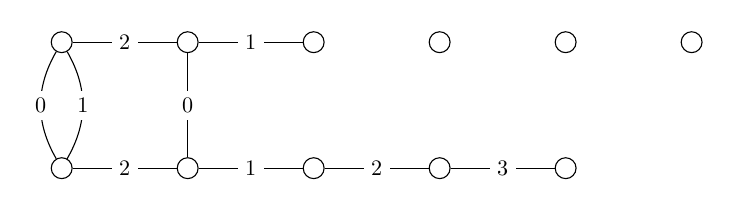
\begin{tikzpicture}[scale=.8]

        \begin{scope}[every node/.style={circle,draw, transform shape}]
          \node (1)  at (0,0) {};
          \node (2)  at (0,2) {};
          \node (3)  at (2,0) {};
          \node (4)  at (2,2)  {};
          \node (5)  at (4,0)  {};
          \node (6)  at (4,2)  {};
          \node (7)  at (6,2)  {};
          \node (8)  at (8,2)  {};
          \node (9)  at (10,2) {};
          \node (10) at (6,0)  {};
          \node (11) at (8,0)  {};
        \end{scope}

        \begin{scope}[every node/.style={fill=white, transform shape}]

          \begin{scope}[every edge/.style={draw}]
            \path (1)  edge[bend left=30] node {$0$} (2);
            \path (3)  edge node {$0$} (4);
            \path (3)  edge node {$1$} (5);
            \path (4)  edge node {$1$} (6);
            \path (1)  edge[bend right=30] node {$1$} (2);
            \path (1)  edge node {$2$} (3);
            \path (2)  edge node {$2$} (4);
            \path (5)  edge node {$2$} (10);
            \path (10) edge node {$3$} (11);
          \end{scope}
        \end{scope}

      \end{tikzpicture}
      \caption{}
    \end{center}
  \end{figure}

  \begin{figure}[H]
    \begin{center}
      \begin{tikzpicture}[scale=.8]

        \begin{scope}[every node/.style={circle,draw, transform shape}]
          \node (1)  at (0,0) {};
          \node (2)  at (0,2) {};
          \node (3)  at (2,0) {};
          \node (4)  at (2,2)  {};
          \node (5)  at (4,0)  {};
          \node (6)  at (6,0)  {};
          \node (7)  at (8,0)  {};
          \node (8)  at (10,0)  {};
          \node (9)  at (12,0)  {};
          \node (10) at (14,0)  {};
          \node (11) at (16,0)  {};
        \end{scope}

        \begin{scope}[every node/.style={fill=white, transform shape}]

          \begin{scope}[every edge/.style={draw}]
            \path (1)  edge[bend left=30] node {$0$} (2);
            \path (3)  edge node {$0$} (4);
            \path (3)  edge node {$1$} (5);
            \path (1)  edge[bend right=30] node {$1$} (2);
            \path (1)  edge node {$2$} (3);
            \path (2)  edge node {$2$} (4);
            \path (9)  edge node {$2$} (10);
            \path (10) edge node {$3$} (11);
          \end{scope}
        \end{scope}

      \end{tikzpicture}
      \caption{}
    \end{center}
  \end{figure}

  \paragraph{}
  In the first case the other $\rho_3$ edge must be at the end of another branch and linked be a $\rho_2$ edge and a $\rho_1$ edge. But then there are a vertex and a $\rho_1$ edge that cannot be placed.

  \paragraph{}
  In the second case, the other $\rho_3$ edge must be placed next to the $\rho_2$ edge and one $\rho_1$ edge cannot be placed.

  \paragraph{}
  If the double edge is $(\rho_1, \rho_2)$, the alternating square must be $[\rho_0, \rho_2]$ (up to duality).

  \begin{figure}[H]
    \begin{center}
      \begin{tikzpicture}[scale=.8]

        \begin{scope}[every node/.style={circle,draw, transform shape}]
          \node (1)  at (0,0) {a};
          \node (2)  at (0,2) {b};
          \node (3)  at (2,0) {c};
          \node (4)  at (2,2)  {d};
          \node (5)  at (4,0)  {};
          \node (6)  at (6,0)  {};
          \node (7)  at (8,0)  {};
          \node (8)  at (10,0)  {};
          \node (9)  at (12,0)  {};
          \node (10) at (14,0)  {};
          \node (11) at (16,0)  {};
        \end{scope}

        \begin{scope}[every node/.style={fill=white, transform shape}]

          \begin{scope}[every edge/.style={draw}]
            \path (1)  edge node {$0$} (3);
            \path (2)  edge node {$0$} (4);
            \path (1)  edge[bend left=30] node {$1$} (2);
            \path (3)  edge node {$2$} (4);
            \path (1)  edge[bend right=30] node {$2$} (2);
          \end{scope}
        \end{scope}

      \end{tikzpicture}
      \caption{}
    \end{center}
  \end{figure}

  \paragraph{}
  Now only single edge can be placed. Thus the alternating square can only be connected by $c$ or $d$. There are only two $\rho_2$ edges to connect two $\rho_3$ edges. Thus the patterns saw in Proposition~\ref{rho0atEnd} must be used\footnote{Not complete}. In every case, using one pattern consume leave $\rho_1$ edges. But the $\rho_1$ edges cannot be used to link all the component $\rho_1$ due to the limitations of Proposition~\ref{fixed-only-1}.

  \paragraph{}
  If the difference of the indices is 3, the double edge must be $(\rho_0, \rho_3)$ but the adjacent square must be $[\rho_1, \rho_3]$. There is a single $\rho_0$ edge remaining, this edge must be adjacent to a $\rho_1$ edge. There is only one $\rho_1$ edge for 4 $\rho_2$ edges, hence the graph can never be connected. Thus the index of the double edge must be separated by 2 and the double edge is $(\rho_0, \rho_2)$.\footnote{Not complete}

  \paragraph{}
  No index 0 or 3 can be repeated in both patterns if they are distinct because the alternating square uses two edges. But $\rho_0$ and $\rho_3$ are 2-transpositions and thus have only two edges.

\end{proof}

\begin{lemma}
  If there are two alternating squares then they must be $[\rho_0, \rho_2]$ and $[\rho_1, \rho_3]$.
\end{lemma}

\begin{proof}
  The alternating square uses two edges. Thus the involutions $\rho_0$ or $\rho_3$ cannot be used in both squares.

  \paragraph{}
  If the indices of an alternating square are consecutive, another alternating square must be adjacent to the first one by Lemma~\ref{continue-alternating-square}. Thus all squares have been placed. There are two possibilities: $[\rho_0, \rho_1]$ or $[\rho_1, \rho_2]$. In the first case, there are no possible adjacent squares because $[\rho_0, \rho_2]$ would use three $\rho_0$ edges and $[\rho_1, \rho_1]$ does not make sens by Proposition~\ref{fixed-only-1}. In the second case, the only possibility for an adjacent square is $[\rho_0, \rho_2]$. Now no extra alternating square can be built and thus this last square must be connected by a single edge.

  \begin{figure}[H]
    \begin{center}
      \begin{tikzpicture}[scale=.8]

        \begin{scope}[every node/.style={circle,draw, transform shape}]
          \node (1)  at (0,0) {};
          \node (2)  at (0,2) {};
          \node (3)  at (2,0) {};
          \node (4)  at (2,2)  {};
          \node (5)  at (4,0)  {};
          \node (6)  at (4,2)  {};
          \node (7)  at (6,0)  {};
          \node (8)  at (8,0)  {};
          \node (9)  at (10,0)  {};
          \node (10) at (12,0)  {};
          \node (11) at (14,0)  {};
        \end{scope}

        \begin{scope}[every node/.style={fill=white, transform shape}]

          \begin{scope}[every edge/.style={draw}]
            \path (5)  edge node {$0$} (3);
            \path (6)  edge node {$0$} (4);
            \path (1)  edge node {$1$} (3);
            \path (2)  edge node {$1$} (4);
            \path (5)  edge node {$1$} (7);
            \path (1)  edge node {$2$} (2);
            \path (3)  edge node {$2$} (4);
            \path (5)  edge node {$2$} (6);
          \end{scope}
        \end{scope}

      \end{tikzpicture}
      \caption{}
    \end{center}
  \end{figure}

  \paragraph{}
  Now there two $\rho_3$ that are not part of an alternating square for only one $\rho_2$ but that is forbidden by Lemma~\ref{rho0atEnd}.

  \paragraph{}
  If the difference between the indices if 3, the square is $[\rho_0, \rho_3]$. The adjacent square must be $[\rho_1, \rho_3]$ up to duality. But the index $3$ is repeated and that is impossible.

  \paragraph{}
  Thus one alternating square must be $[\rho_0, \rho_2]$ and the other must be $[\rho_1, \rho_3]$.

\end{proof}

Now we list all the possible monodromy groups with rank 4 on $A_{11}$.

\begin{theorem}
  All monodromy groups of rank 4 on $A_{11}$ with two 4-transpositions are those presented in appendix~\ref{rank4-2-4transpositions} (p.~\pageref{rank4-2-4transpositions})).
\end{theorem}

\paragraph{}
The proof of this theorem is left to the reader because it is just a very simple (but long) application of the Method~\ref{method}.

\paragraph{}
There are a lot of monodromy groups, thus it is important to be systematic. The appendix~\ref{rank4-2-4transpositions} is structured in the following way and we encourage the reader to search for all monodromy groups in the same way.

\begin{enumerate}
  \item Choose which structures consume the "joker" edges: two double edges, one double edge and one alternating square or two alternating squares.
  \item Choose the length of the chain between the two structures.
  \item Choose the distance between one structure and the end of the graph.
\end{enumerate}

\paragraph{}
Once this decision tree is made, finding the graphs is very easy. The structure of appendix~\ref{rank4-2-4transpositions} matches this decision tree. It's important to check that the dual of the current graph has not already be found.

\paragraph{}
For each of this monodromy group we prove that it is not a string C-group representation of $A_{11}$. We make three sub-sections for the three main cases. The proofs are not complete. In the first examples a method is given to proof that the monodromy group is not a string C-group representation.

\subsection{Two double edges}

\begin{theorem}
  None of the monodromy groups with two double edges presented in appendix~\ref{rank4-2-1-4transpositions} are not string C-groups representation of $A_{11}$.
\end{theorem}

\begin{proof}
  For all the graphs we always consider $S_1 = \{\rho_1,\rho_2,\rho_3\}$ and $S_2 = \{\rho_2, \rho_3, \rho_4\}$. We must prove that $\Gamma_{S_1 \cap S_2} \neq \Gamma_{S_1} \cap \Gamma_{S_2}$.

  \paragraph{}
  We look at the first graph, the Figure~\ref{r4-1-1}. Here is one copy of this graph.

  \begin{figure}[H]
    \begin{center}
      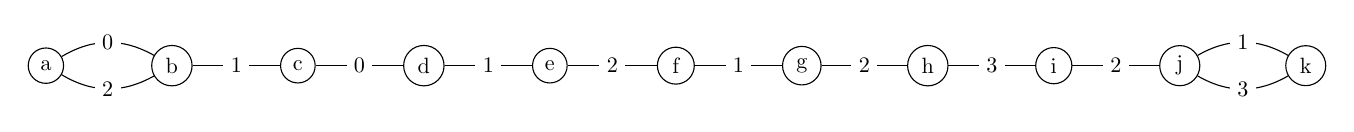
\begin{tikzpicture}[scale=.8]

        \begin{scope}[every node/.style={circle,draw, transform shape}]
          \node (1)  at (0,0) {a};
          \node (2)  at (2,0) {b};
          \node (3)  at (4,0) {c};
          \node (4)  at (6,0)  {d};
          \node (5)  at (8,0)  {e};
          \node (6)  at (10,0)  {f};
          \node (7)  at (12,0)  {g};
          \node (8)  at (18,0)  {j};
          \node (9)  at (20,0)  {k};
          \node (10) at (16,0)  {i};
          \node (11) at (14,0)  {h};
        \end{scope}

        \begin{scope}[every node/.style={fill=white, transform shape}]

          \begin{scope}[every edge/.style={draw}]
            \path (1)  edge[bend left=30] node {$0$} (2);
            \path (3)  edge node {$0$} (4);
            \path (2)  edge node {$1$} (3);
            \path (4)  edge node {$1$} (5);
            \path (6)  edge node {$1$} (7);
            \path (8)  edge[bend left=30] node {$1$} (9);
            \path (1)  edge[bend right=30] node {$2$} (2);
            \path (5)  edge node {$2$} (6);
            \path (7)  edge node {$2$} (11);
            \path (8)  edge node {$2$} (10);
            \path (8)  edge[bend right=30] node {$3$} (9);
            \path (10) edge node {$3$} (11);
          \end{scope}
        \end{scope}

      \end{tikzpicture}
      \caption{}
    \end{center}
  \end{figure}

  \paragraph{}
  Let's have a look at $\Gamma_{S_1}$ and $\Gamma_{S_2}$

  \begin{figure}[H]
    \begin{center}
      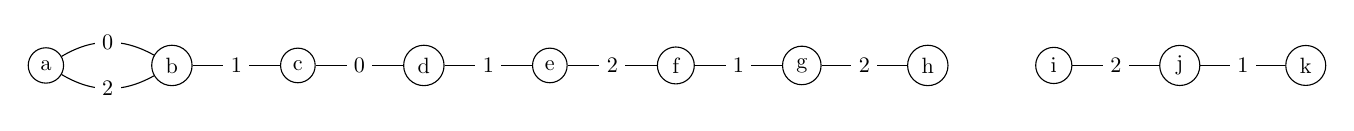
\begin{tikzpicture}[scale=.8]

        \begin{scope}[every node/.style={circle,draw, transform shape}]
          \node (1)  at (0,0) {a};
          \node (2)  at (2,0) {b};
          \node (3)  at (4,0) {c};
          \node (4)  at (6,0)  {d};
          \node (5)  at (8,0)  {e};
          \node (6)  at (10,0)  {f};
          \node (7)  at (12,0)  {g};
          \node (8)  at (18,0)  {j};
          \node (9)  at (20,0)  {k};
          \node (10) at (16,0)  {i};
          \node (11) at (14,0)  {h};
        \end{scope}

        \begin{scope}[every node/.style={fill=white, transform shape}]

          \begin{scope}[every edge/.style={draw}]
            \path (1)  edge[bend left=30] node {$0$} (2);
            \path (3)  edge node {$0$} (4);
            \path (2)  edge node {$1$} (3);
            \path (4)  edge node {$1$} (5);
            \path (6)  edge node {$1$} (7);
            \path (8)  edge node {$1$} (9);
            \path (1)  edge[bend right=30] node {$2$} (2);
            \path (5)  edge node {$2$} (6);
            \path (7)  edge node {$2$} (11);
            \path (8)  edge node {$2$} (10);
          \end{scope}
        \end{scope}

      \end{tikzpicture}
      \caption{$\Gamma_{S_1}$}
    \end{center}
  \end{figure}

  \begin{figure}[H]
    \begin{center}
      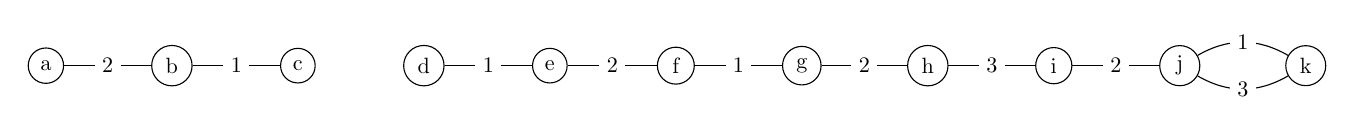
\begin{tikzpicture}[scale=.8]

        \begin{scope}[every node/.style={circle,draw, transform shape}]
          \node (1)  at (0,0) {a};
          \node (2)  at (2,0) {b};
          \node (3)  at (4,0) {c};
          \node (4)  at (6,0)  {d};
          \node (5)  at (8,0)  {e};
          \node (6)  at (10,0)  {f};
          \node (7)  at (12,0)  {g};
          \node (8)  at (18,0)  {j};
          \node (9)  at (20,0)  {k};
          \node (10) at (16,0)  {i};
          \node (11) at (14,0)  {h};
        \end{scope}

        \begin{scope}[every node/.style={fill=white, transform shape}]

          \begin{scope}[every edge/.style={draw}]
            \path (2)  edge node {$1$} (3);
            \path (4)  edge node {$1$} (5);
            \path (6)  edge node {$1$} (7);
            \path (8)  edge[bend left=30] node {$1$} (9);
            \path (1)  edge node {$2$} (2);
            \path (5)  edge node {$2$} (6);
            \path (7)  edge node {$2$} (11);
            \path (8)  edge node {$2$} (10);
            \path (8)  edge[bend right=30] node {$3$} (9);
            \path (10) edge node {$3$} (11);
          \end{scope}
        \end{scope}

      \end{tikzpicture}
      \caption{$\Gamma_{S_2}$}
    \end{center}
  \end{figure}

  \paragraph{}
  In the graph of $\Gamma_{S_1}$, the group of the left component is $S_8$ and the group of the right component is $S_3$ but because the global group must only have even permutation in order to have $A_{11}$, there is a semi-direct product and the group is $A_8 : S_3$.

  \paragraph{}
  The goal is now to prove that $\Gamma_{S_1} \cap \Gamma_{S_2} \ge S_5$.

  \paragraph{}
  In the group $\Gamma_{S_1}$ we leave the points $i,j,k$ fixed for now. This is an even permutation on those three points. The group of the left component is one of the lateral class of $A_8$ but because the permutation on $i,j,k$ is even, it is $A_8$. Thus it contains all the permutations of $d,e,f,g,h$, i.e. $S_5$ on those five points. If the permutation on $d,e,f,g,h$ is odd, it is sufficient to permute two points in $a,b,c$ in order to have a permutation of $A_8$.

  \paragraph{}
  Now we look at $\Gamma_{S_2}$. We need to prove that all the permutations of $d,e,f,g,h$ are also in this group. First for every permutation of the points $a,b,c$ in $\Gamma_{S_1}$ the same permutation can be made in $\Gamma_{S_2}$ because the group of permutations of those 3 points is $S_3$ on $\Gamma_{S_2}$. The parity of the permutation of the component $d,e,f,g,h,i,j,k$ must be the same as the parity of the permutation of $a,b,c$ and that is possible because the points $i,j,k$ are fixed. Thus it means that the parity of the permutation on $d,e,f,g,h$ in $\Gamma_{S_2}$ is the same as in $\Gamma_{S_1}$. Thus the group of permutations on $d,e,f,g,h$ in $\Gamma_{S_2}$ is one coset of $A_5$ but the permutation applied in $\Gamma_{S_1}$ lies in this coset.

  \paragraph{}
  Thus the intersection is at least $S_5$ but $\Gamma_{S_1 \cap S_2} = D_{24}$ and $D_{24} \neq S_5$. The graph is therefore not a string C-group representation.

  \paragraph{}
  The same kind of reasoning can be made for all graphs of Appendix~\ref{rank4-2-1-4transpositions}. The results are displayed in Table~\ref{results-2-1}.

\begin{table}
  \centering
  \begin{tabular}{|c|c|c|c|c|c|c|}
    \hline
    Figure & $\Gamma_{S_1}$ & $\Gamma_{S_2}$ & $\Gamma_{S_1 \cap S_2}$ & $\#\Gamma_{S_1 \cap S_2}$ & $\Gamma_{S_1} \cap \Gamma_{S_2}$ & $\#(\Gamma_{S_1} \cap \Gamma_{S_2})$ \\ \hline
    \ref{r4-1-1} & $A_8 : S_3$ & $A_8 : S_3$ & $D_{30}$ & 30 & $\ge S_5$ & $\ge 120$ \\ \hline
    \ref{r4-1-2} & $A_5 \times D_{10}$ & $A_8 : S_3$ & $D_{30}$ & 30 & $\ge S_3 \times D_{10}$ & $\ge 60$ \\ \hline
    \ref{r4-1-3} & $A_7 : S_4$ & $A_7 : S_4$ & $D_{24}$ & 24 & $\ge S_4 \times S_4$ & $\ge 576$ \\ \hline
    \ref{r4-1-4} & $A_7 : D_8$ & $A_7 : D_8$ & $D_{24}$ & 24 & $\ge D_8 \times D_8$ & $\ge 64$ \\ \hline
    \ref{r4-1-5} & $A_8 : S_3$ & $A_5 \times D_{10}$ & $D_{30}$ & 30 & $\ge S_3 \times D_{10}$ & $\ge 60$ \\ \hline
    \ref{r4-1-6} & $A_8 : S_3$ & $A_{10}$ & $D_{42}$ & 42 & $\ge S_7$ & $\ge 5040$ \\ \hline
    \ref{r4-1-7} & $A_5 \times D_{10}$ & $A_{10}$ & $D_{10}$ & 10 & $\ge D_{10} \times D_{10}$ & $\ge 100$ \\ \hline
    \ref{r4-1-8} & $A_{10}$ & $A_{10}$ & $D_{18}$ & 18 & $\ge A_9$ & $\ge 181400$ \\ \hline
    \ref{r4-1-9} & $A_{10}$ & $A_5 \times D_{10}$ & $D_{10}$ & 10 & $\ge D_{10} \times D_{10}$ & $\ge 100$ \\ \hline
    \ref{r4-1-10}& $A_7 : D_8$ & $S_9$ & $D_{40}$ & 40 & $\ge S_5$ & $\ge 120$ \\ \hline
    \ref{r4-1-11}& $A_{10}$ & $A_5 : S_6$ & $D_{10}$ & 10 & $\ge S_5$ & $\ge 120$ \\ \hline
    \ref{r4-1-12}& $S_9$ & $A_7 :S_4$ & $D_{40}$ & 40 & $\ge S_5$ & $\ge 120$ \\ \hline
    \ref{r4-1-13}& $A_8 : S_3$ & $A_8 : S_3$ & $D_{30}$ & 30 & $\ge S_5$ & $\ge 120$ \\ \hline
    \ref{r4-1-14}& $A_8 : S_3$ & $A_{10}$ & $D_{42}$ & 42 & $\ge S_7$ & $\ge 5040$ \\ \hline
    \ref{r4-1-15}& $A_{10}$ & $A_{10}$ & $D_{18}$ & 18 & $\ge A_9$ & $\ge 181400$ \\ \hline
    \ref{r4-1-16}& $S_9$ & $S_9$ & $D_{28}$ & 28 & $\ge S_7$ & $\ge 5040$ \\ \hline
    \ref{r4-1-17}& $A_{10}$ & $A_8 : S_3$ & $D_{42}$ & 42 & $\ge S_7$ & $\ge 5040$ \\ \hline
    \ref{r4-1-18}& $A_{10}$ & $A_{10}$ & $D_{18}$ & 18 & $\ge A_9$ & $\ge 181440$ \\ \hline
    \ref{r4-1-19}& $A_{10}$ & $A_7 : S_4$ & $D_{42}$ & 42 & $\ge S_7$ & $\ge 5040$ \\ \hline
    \ref{r4-1-20}& $S_9$ & $A_5 : S_6$ & $D_{12}$ & 12 & $\ge S_6$ & $\ge 720$ \\ \hline
    \ref{r4-1-21}& $A_7 : S_{4}$ & $A_{10}$ & $D_{42}$ & 42 & $\ge S_7$ & $\ge 5040$ \\ \hline

  \end{tabular}
  \caption{}
  \label{results-2-1}
\end{table}

\subsection{One double edge and one alternating square}

  \paragraph{}
  The same process can be done with the monodromy groups of Appendix~\ref{rank4-2-2-4transpositions}. The result is displayed in Table~\ref{results-2-2}.

  \begin{table}
    \centering
    \begin{tabular}{|c|c|c|c|c|c|c|}
      \hline
      Figure & $\Gamma_{S_1}$ & $\Gamma_{S_2}$ & $\Gamma_{S_1 \cap S_2}$ & $\#\Gamma_{S_1 \cap S_2}$ & $\Gamma_{S_1} \cap \Gamma_{S_2}$ & $\#(\Gamma_{S_1} \cap \Gamma_{S_2})$ \\ \hline

      \ref{r4-2-1} & $A_8 : S_3$ & $A_8 : S_3 $ & $D_{30}$ & 30 & $\ge S_5$ & $\ge 120$ \\ \hline
      \ref{r4-2-2} & $A_7 : D_8$ & $A_8 : S_3$ & $D_{24}$ & 24 & & \\ \hline
      \ref{r4-2-3} & $A_8 : S_3$ & $A_8 : S_3 $ & $D_{30}$ & 30 & $\ge S_5$ & $\ge 120$ \\ \hline
      \ref{r4-2-4} & $A_8 : S_3$ & $A_{10}$ & $D_{42}$ & 42 & $\ge S_7$ & $\ge 5040$ \\ \hline
      \ref{r4-2-5} & $A_7 : D_8$ & $A_{10}$ & $D_{24}$ & 24 & & \\ \hline
      \ref{r4-2-6} & $A_8 : S_3$ & $A_{10}$ & $D_{42}$ & 42 & $\ge S_7$ & $\ge 5040$ \\ \hline
      \ref{r4-2-7} & \\ \hline
      \ref{r4-2-8} & \\ \hline
      \ref{r4-2-9} & \\ \hline
      \ref{r4-2-10} & \\ \hline
      \ref{r4-2-11} & \\ \hline
      \ref{r4-2-12} & \\ \hline
        \end{tabular}
    \caption{}
    \label{results-2-2}
  \end{table}

\subsection{Two alternating squares}
  \paragraph{}
  This section can be done very easily by doing the same procedure that for the previous one. The results are displayed in Table~\ref{results-2-3}

  \begin{table}
    \centering
    \begin{tabular}{|c|c|c|c|c|c|c|}
      \hline
      Figure & $\Gamma_{S_1}$ & $\Gamma_{S_2}$ & $\Gamma_{S_1 \cap S_2}$ & $\#\Gamma_{S_1 \cap S_2}$ & $\Gamma_{S_1} \cap \Gamma_{S_2}$ & $\#(\Gamma_{S_1} \cap \Gamma_{S_2})$ \\ \hline

      \ref{r4-3-1} & $S_9$ & $S_9$ & $D_{28}$ & 28 & $\ge S_7$ & $\ge 5040$ \\ \hline
      \ref{r4-3-2} & $S_3 \times S_3 \times S_3:S_3$ & $A_8 : S_3$ & $D_{12}$ & 12 & & \\ \hline
      \ref{r4-3-3} & $S_9$ & $S_9$ & $D_{28}$ & 28 & $\ge S_7$ & $\ge 5040$ \\ \hline
      \ref{r4-3-4} & $A_8 : S_3$ & $A_8 : S_3$ & $D_{30}$ & 30 & $\ge S_5$ & $\ge 120$ \\ \hline
      \ref{r4-3-5} & $A_8 : S_3$ & $A_8 : S_3$ & $D_{30}$ & 30 & $\ge S_5$ & $\ge 120$ \\ \hline
      \ref{r4-3-6} & $A_8 : S_3$ & $S_9$ & $D_{12}$ & 12 & $\ge S_6$ & $\ge 720$ \\ \hline
      \ref{r4-3-7} & $A_8 : S_3$ & $A_8 : S_3$ & $D_{30}$ & 30 & $\ge S_5$ & $\ge 120$  \\ \hline
      \ref{r4-3-8} & $A_7 \times 2 \cdot 2 : 2$ & $S_9$ & $D_{40}$ & 40 & $\ge S_5$ & $\ge 120$ \\ \hline
      \ref{r4-3-9} & $S_7 \times 2:2$ & $S_9$ & $D_{40}$ & 40 & $\ge S_5$ & $\ge 120$ \\ \hline
      \ref{r4-3-10}& $S_9$ & $S_9$ & $D_{28}$ & 28 & $\ge S_7$ & $\ge 720$ \\ \hline

    \end{tabular}
    \caption{}
    \label{results-2-3}
  \end{table}

\end{proof}
